\subsection{Construcción de memorias}
Cuando surge la pregunta: ¿Cuantos chips de memoria se necesitan para almacenar $1K$ palabras de $16$ bits cada una? La respuesta es: $1K \times 16 = 16K$ bits. Si cada chip de memoria tiene $1K$ bits, entonces se necesitan $16$ chips.

\begin{mdframed}[backgroundcolor=gray!10,linewidth=0]
    Para generalizar, si se tienen $m$ palabras de $n$ bits cada una, se necesitan $m \times n$ bits. Si cada chip de memoria tiene $k$ bits, entonces se necesitan $\frac{m \times n}{k}$ chips.
\end{mdframed}

\newpage
\subsubsection{Tamaño de la memoria y dirección}
La cantidad de bits de una memoria se calcula como $2^{\text{dirección}} \times \text{tamaño de palabra}$. Por ejemplo, si se tiene una memoria de $16$ palabras de $8$ bits cada una, la cantidad de bits de la memoria es $2^4 \times 8 = 128$ bits. 

Generalmente el gráfico de una memoria se representa de la siguiente manera:

\begin{figure}[h]
    \centering
    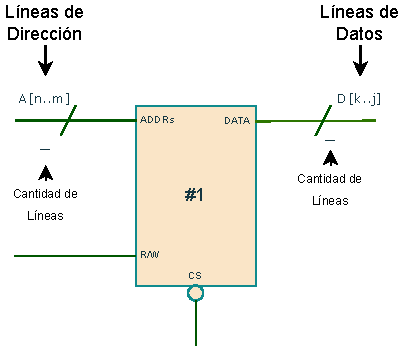
\includegraphics[scale=1]{img/diagramamem.pdf}
    \caption{Diagrama de una memoria}
\end{figure}
Donde de la cantidad de líneas de dirección se obtiene la cantidad de palabras y de la cantidad de líneas de datos se obtiene el tamaño de la palabra.
